\newpage
{\bfseries MPHTИ 52.13.15}

\sectionwithauthors{А.С. Кайназаров, В.Ф. Демин, А.С. Кайназарова,  Е.А.Абрахман}{ДАЙЫНДЫҚ ТАУ-КЕН ЖҰМЫСТАРЫНЫҢ АЙНАЛАСЫНДАҒЫ СИЫМДЫ ЖЫНЫСТАРДЫҢ ЖЫЛЖУЫН МОДЕЛЬДЕУ}

\begin{center}
{\bfseries \textsuperscript{1}А.С. Кайназаров\textsuperscript{🖂},
\textsuperscript{2}В.Ф. Демин, \textsuperscript{1,}А.С. Кайназарова,
\textsuperscript{2} Е.А.Абрахман}

\textsuperscript{1}Академик Қ. Сәтбаев атындағы Екібастұз
инженерлік-техникалық институты,

Екібастұз, Қазақстан,

\textsuperscript{2}Әбілқас Сағынов атындағы Қарағанды техникалық
университеті, Қарағанды, Қазақстан,

{\bfseries \textsuperscript{🖂}} Корреспондент-автор: armanayn@mail.ru
\end{center}

Аналитикалық негіздеу үшін тау-кен геологиялық, тау-кен-техникалық және
технологиялық пайдалану жағдайларының әсерінен жұмыстарды жүргізу және
ұстаудың геомеханикалық шарттарын ескере отырып, тау-кен массасының
кернеулі-деформациялық күйін модельдеудің сандық әдістемесі ұсынылған.
кен қазбаларының айналасында негізгі жыныстардың жылжуын модельдеу.
Дайындық тау-кен қазбаларының айналасында орналасқан жыныстардың жылжуын
аналитикалық модельдеу (анықтау) үшін келесі әрекеттер орындалады:
қазбаны жүргізудің геологиялық шарттары анықталады, ол үшін топырақ пен
шатыр жыныстарын көрсете отырып, геологиялық кесу жасалады; тау
жыныстары қабаттарының механикалық сипаттамаларына талдау жасалады;
тазарту қазбасының маңында-- кенжардың алдында, өңдеу және өңдеу
аймағында кернеулердің сызықтары мен диаграммаларын салу орындалады
қалдық тірек қысымы аймағында; тазарту қазбасының ықпалынан тыс қазбаның
айналасындағы тау жыныстарының серпімді емес деформацияларының аймағын
есептеу және алдыңғы уақыттағы ұқсас жағдайлардағы бақылаулардың
эксперименттік деректері негізінде орын ауыстыру жылдамдықтарының
диаграммасын құру және осы тау-кен қазбасының бүкіл қызмет ету
кезеңіндегі орын ауыстыру жылдамдықтарының диаграммаларын құру, ұқсас
игеру жағдайлары үшін қолда бар тәжірибелік деректерді жалпылау арқылы
белгіленген орын ауыстыруларды ескере отырып жүргізіледі.

{\bfseries Түйін сөздер:} тау-кен қазбалары, бекіту параметрлері,
геомеханикалық процесстер, анкер бекіткіші, технологиялық схемалар,
аналитикалық модельдеу, тау қысымы, тау жыныстарының жылжуы.

\begin{center}
{\large\bfseries МОДЕЛИРОВАНИЕ СМЕЩЕНИЙ ВМЕЩАЮЩИХ ПОРОД ВОКРУГ ПОДГОТОВИТЕЛЬНЫХ
ГОРНЫХ ВЫРАБОК}

{\bfseries \textsuperscript{1}А.С. Кайназаров\textsuperscript{🖂},
\textsuperscript{2}В.Ф.Демин, \textsuperscript{1} А.С. Кайназарова,
\textsuperscript{2}Е.А. Абрахман}

\textsuperscript{1}Екибастузский инженерно-технический институт имени
академика К. Сатпаева, Экибастуз, Казахстан,

\textsuperscript{2}Карагандинский технический университет имени Абылкаса
Сагинова, Караганда, Казахстан,

e-mail: armanayn@mail.ru
\end{center}

Предложена численная методика моделирования напряженно-деформированного
состояния массива горных пород с учетом геомеханических условий
проведения и поддержания выработки при влиянии горно-геологических,
горно-технических и технологических условий эксплуатации схем ведения
горных работ для аналитического обоснования моделирование смещений
вмещающих пород вокруг подготовительных горных выработок. Для
аналитического моделирования (определения) смещений вмещающих пород
вокруг подготовительных горных выработок выполняются следующие действия:
определяются геологические условия проведения выработки, для чего
составляется геологический разрез с указанием пород почвы и кровли;
производится анализ механических характеристик слоев пород; выполняется
построение изолиний и эпюр напряжений в окрестности очистной выработки--
впереди забоя, в зоне подработки и в зоне остаточного опорного давления;
производится расчет зоны неупругих деформаций пород вокруг выработки вне
влияния очистной выработки и построение эпюры скоростей смещений на
основе экспериментальных данных наблюдений в аналогичных условиях в
предшествующее время и построение эпюр скоростей смещений на весь период
службы данной горной выработки с учетом установленных смещений путем
обобщения имеющихся опытных данных для аналогичных условий разработки.

{\bfseries Ключевые слова:} горные выработки, параметры крепления,
геомеханические процессы, анкерная крепь, технологические схемы,
аналитическое моделирование, горное давление, сдвижение пород.

\begin{center}
{\large\bfseries MODELING OF DISPLACEMENTS OF HOST ROCKS AROUND PREPARATORY MINE WORKINGS}

{\bfseries \textsuperscript{1}А.S. Kainazarov\textsuperscript{🖂},
\textsuperscript{2}V.F. Dеmin, \textsuperscript{1}А.S. Kainazarova,
\textsuperscript{2}E.A. Abdrachman}

\textsuperscript{1}Ekibastuz technical and engineering institute named
after the academician K.Satpayev,

Ekibastuz, Kazakhstan,

\textsuperscript{2}Abylkas Saginov Karaganda Technical University,
Kazakhstan,

armanayn@mail.ru
\end{center}

A numerical method for modeling the stress-strain state of a rock mass
is proposed, taking into account the geomechanical conditions of
conducting and maintaining mining under the influence of mining, mining,
technical and technological operating conditions of mining schemes for
analytical justification of modeling displacements of host rocks around
preparatory mine workings. For analytical modeling (determination) of
displacements of the host rocks around the preparatory mine workings,
the following actions are performed: the geological conditions of the
workings are determined, for which a geological section is made
indicating the soil and roof rocks; the mechanical characteristics of
the rock layers are analyzed; isolines and stress plots are constructed
in the vicinity of the treatment workings -- ahead of the face, in the
work area and in the area of residual reference pressure; the
calculation of the zone of inelastic deformations of rocks around the
mine is carried out outside the influence of the treatment mine and the
plotting of displacement velocities based on experimental observation
data under similar conditions in the previous time and the plotting of
displacement velocities for the entire service life of this mine, taking
into account the established displacements, by generalizing the
available experimental data for similar development conditions.

{\bfseries Keywords}: mining, fastening parameters, geomechanical
processes, anchorage, technological schemes, analytical modeling, rock
pressure, rock displacement.

\begin{multicols}{2}
{\bfseries Кіріспе.} Тау қысымының ең көп таралған түрлерінің бірі --
қоршаған тау-кен өндірісінің жойылуы. Ол массивтің едәуір көлемін қамтуы
мүмкін, нәтижесінде жойылған жыныстардың бір бөлігі өз салмағының
әсерінен өндіріске құлайды. Қирау аймағының кішігірім мөлшерінде тау
қысымы тау жыныстарының жекелеген бөліктерінің құлауында көрінеді. Оның
көрінуінің тағы бір түрі -- пайдалану кезінде байқалатын өндіріс
контурының деформациясы. Көбінесе көріністердің екі түрі де бір мезгілде
байқалады, ал ең қауіпті формалар динамикалық болып табылады: күшті тау
жыныстарына тән нәзік бұзылатын тау жыныстарының «атуы», кенеттен
шығарындылар мен тау соққылары. Контурға жақын жыныстар ұзақ жүктемелер
кезінде дамудың үлкен тереңдігінде серпімді жүктеме режимінен серпімді
емес деформация сатысына өтеді. Бұл кезеңде массивтің тұтастығы
бұзылады, микро ақаулар пайда болады, олар болашақта макрожарылуларға
айналады. Көрсетілген деформациялардың ұлғаюына байланысты (кеңею) тау
жыныстарының көлемінің ұлғаюы байқалады, оның мәні серпімді
деформациялардан туындаған орын ауыстырулардан үлкен. Эксперименттік
алынған деректерді ескере отырып, өндіріс контурының болжамды жылжуын
модельдеу жүргізілді.

Жер асты құрылымының жанындағы тау-кен жұмыстары кезінде тау-кен
массасының бұзылуы белгілі бір уақытта кернеу-деформациялық күй
параметрлерінің белгілі бір комбинациясы белгілі бір сындық мәнге жеткен
кезде болады.

Тау-кен жұмыстарының тау-кен және технологиялық факторларын ескере
отырып, кен қазбаларының контурлық массивінің жылжуын есептеу
бағдарламасының алгоритмін құру үшін оның теориялық негіздемесі төменде
келтірілген.

Өндірістердің контурларының ығысу жылдамдығы олардың маңындағы тау
жыныстары массивінің созылу дәрежесіне және массивтің
физикалық-механикалық қасиеттеріне байланысты. Өңдеу жұмыстарының
контурларының жылжуын есептеу үшін олардың тау-кен жағдайларының
өзгеруімен анықталатын жылдамдықтарын пайдалану керек.

\emph{Зерттеудің мақсаты.} Тау жыныстары қысымының көріністерін болжау
әдістемесін әзірлеу және әлсіз негізгі жыныстары бар кен орындарында
көмір қорын өндіру кезінде жұмыс беттеріндегі шатырды басқарудың
техникалық шешімдерін жетілдіру.

\emph{Зерттеу мақсаттары.} Өндірістік беткейлердегі тау жыныстары
қысымының көріністерінің параметрлерін анықтау. Ұзын қабырғалы шатырдың
жүктеме қасиеттеріне және оның тұрақтылығына тау жыныстарының қысымының
жоғарылауының әсер ету механизмі жеткілікті түрде зерттелмеген, бұл ұзын
қабырға беттеріндегі шатырды басқару бойынша тиімді шешімдер қабылдауға
әрқашан мүмкіндік бермейді. Эксперименттік алынған мәліметтерді ескере
отырып, қазба контурының болжамды жылжуын есептеу.

\emph{Ғылыми жұмыстың жаңалығы.} Жүргізілген зерттеулер жұмыс
қабаттарындағы тау жыныстары қысымының көріністерін болжау, тау-кен
жұмыстарын ұтымды жоспарлау бойынша ұсынымдар жасау және жоғары тау
жыныстарының қысымы аймақтарында жұмыс істейтін ұзын қабырғалы
беткейлердегі шатырды басқарудың әзірленген әдістемесін қолдану
перспективаларын көрсетті.

{\bfseries Материалдар мен әдістер.} Өткен қазбадан байқалған тау қысымының
көріністері контур маңындағы массив жыныстарының ығысуы болып табылады.

Тау-кен қазбалары контурының жылжуын есептеу тазарту кенжарын жылжыту
кезінде олардың орналасқан аймағында пайда болатын максималды кернеулер
бойынша жүзеге асырылады. Бұл жағдайда ең үлкен қиындықтар тазарту
кенжарының қозғалыс жылдамдығына және әзірленіп жатқан қабаттан
қашықтыққа байланысты осы максималды кернеулердің әсер ету уақытын
есепке алу болып табылады.

U\textsubscript{сум} қазбалардағы тау жыныстарының жылжуының соңғы
мәндері серпімді U\textsubscript{1} және серпімді емес
U\textsubscript{2} деформациялар есебінен қосылады (1):

\begin{equation}
U_{сум} = U_{1} + U_{2}.
\end{equation}

Серпімді деформациялар формулалар бойынша анықталады (2):

\begin{equation}
\frac{\partial Х_{х}}{\partial х} + \frac{\partial Х_{у}}{\partial у} + Х = 0,\ \frac{\partial Х_{у}}{\partial х} + \frac{\partial Y_{у}}{\partial у} + Y = 0,
\end{equation}

мұнда \(X_{x} = \lambda\theta + 2\mu\frac{\partial u}{\partial x},\)
\(Y_{y} = \lambda\theta + 2\mu\frac{\partial v}{\partial y},\)
\(X_{y} = \mu\left( \frac{\partial v}{\partial x} + \frac{\partial u}{\partial y} \right),\)

\emph{Х, У, Х\textsubscript{х}, У\textsubscript{у}} -- тиімді орын
ауыстырулар векторлары және олардың жүйе

координаттар осі бойынша проекциялары;

μ -- Пуассон коэффициенті;

ν -- кинематикалық тұтқырлық, Н/м\textsuperscript{2};

u -- деформация жылдамдығы, м/сут;

λ -- бүйірлік тарту коэффициенті, r;

θ -- нүктелердің полярлық координаталары.

Шекті күй аймағындағы тау жыныстарының серпімді емес деформациялары
формула бойынша анықталады (3):

\begin{equation}
U_{2} = \frac{S_{зр}}{Р_{выр}}(К_{раз} - 1),
\end{equation}

мұнда \(S_{зр}\)-- серпімді емес деформациялардың шартты аймағының
ауданы, м\textsuperscript{2};

\(Р_{выр}\)-- қазба периметрі, м;

\(К_{раз}\) -- шектен тыс деформация аймағындағы тау жыныстарының
қопсыту

коэффициенті.

Серпімді емес деформациялардың шартты аймағының ауданы жыныстардың
физикалық-механикалық қасиеттеріне және тау-кен өндірісіне жақын жерде
анықтау үшін формулалардан анықталуы керек, тау жыныстары массивінің
кернеулі-деформацияланған күйіне байланысты: таза массивтегі кернеулер
(4); түзілген өндірістен туындаған қосымша кернеулер (5); массивте
әрекет ететін кернеулердің қосындысы (8) формулаларында көрсетілген
{[}1{]}.

\begin{equation}
\left\{\begin{aligned}
 & {\sigma_{r}}^{(0)} = \sigma_{1}(\frac{1 + \lambda}{2} + \frac{1 - \lambda}{2}\cos(2\theta)) \\
 & {\sigma_{\theta}}^{(0)} = \sigma_{1}(\frac{1 + \lambda}{2} + \frac{1 - \lambda}{2}\cos(2\theta)) \\
 & \tau_{r\theta}^{(0)} = - \sigma_{1}\frac{1 - \lambda}{2}\cos(2\theta).
\end{aligned} \right.
\end{equation}

\begin{equation}
\left\{ \begin{aligned}
 & \sigma_{r}^{(1)} + \sigma_{\theta}^{(1)} = 2\lbrack\Phi(z) + Ф(z)\rbrack \\
 & \sigma_{\theta}^{(1)} - \sigma_{r}^{(1)} + 2i\tau_{r\theta}^{(1)} = 2(z\Phi'(z) + \Psi(z)),
\end{aligned} \right.
\end{equation}

мұнда \(\sigma_{1}\) - негізгі тік кернеу, МПа;

\(\lambda\) - бүйірлік аралық коэффициенті; \emph{r};

\(\theta\) - нүктелердің полярлық координаттары.
\end{multicols}

\begin{equation}
z = \omega(\xi) = c_{0}\xi + \frac{c_{1}}{\xi} + \frac{c_{2}}{\xi^{2}} + \frac{c_{3}}{\xi^{3}} + \frac{c_{4}}{\xi^{4}},\omega'(\xi) \neq 0,|\xi| \geq 1
\end{equation}

(5) \(\Phi(z),\Psi(z)\) функцияларының пішіні бар:

\begin{equation}
\left\{ \begin{aligned}
 & \Phi(z) = \frac{1}{4}(\sigma_{1} + \sigma_{2}) - \frac{X + iY}{8\pi(1 - \nu)}\frac{1}{\omega(\xi)} + \Phi_{*}\xi) \\
 & \Psi(z) = \frac{1}{2}(\sigma_{2} - \sigma_{1})e^{- 2ia} + (3 - 4\nu)\frac{X + iY}{8\pi(1 - \nu)}\frac{1}{\omega(\xi)} + \Psi_{*}\xi),
\end{aligned} \right.
\end{equation}

мұнда \(X + iY\) - массивте әрекет ететін күштердің бас векторы
(нәтижелік мән);

\(F_{x} + iF_{y}\), \(\sigma_{1},\sigma_{2}\) - негізгі кернеулер, МПа;

\(\alpha\) - негізгі бағыттың \emph{O\textsubscript{x}} осімен бұрышы.

\[\Phi_{*}(\xi) = \frac{n(\xi)}{m(\xi)}\sigma^{p} + \frac{\xi^{3}}{m(\xi)}\sigma^{\alpha} - \frac{\xi^{5}}{m(\xi)}p_{n - 1}\left( \frac{1}{\xi} \right)\]

\begin{align*}
{\Psi_{*}(\xi) = \frac{\xi^{3}}{m(\xi)}\left\lbrack (c_{0} - c_{1}\xi^{2} - c_{2}\xi^{3} - c_{3}\xi^{4} - c_{4}\xi^{5})\Phi_{*}(\xi) - p_{n - 1}\left( \frac{1}{\xi} \right) + c_{0}\sigma^{p} - \right.\
}\\{- (c_{0}\xi + c_{1}\xi^{3} + c_{2}\xi^{4} + c_{3}\xi^{5} + c_{4}\xi^{6})\Phi_{*}'(\xi) + \left. \ \left( с_{1} + \frac{2с_{2}}{\xi} + \frac{3с_{3}}{\xi^{2}} + \frac{4с_{4}}{\xi^{3}} \right)\sigma^{\alpha} \right\rbrack,}
\end{align*}

\(\sigma^{р} = Р + \frac{1}{2}(\sigma_{1} + \sigma_{2})\),
\(\sigma^{\alpha} = \frac{1}{2}(\sigma_{2} - \sigma_{1})e^{2i\alpha}\),
\(p_{n - 1}\left( \frac{1}{\xi} \right) = - с_{3}\frac{\overline{а_{2}}}{\xi^{2}} - с_{4}\left( \frac{2\overline{а_{2}}}{\xi^{3}} + \frac{\overline{а_{3}}}{\xi^{2}} \right)\),

\(n(\xi) = c_{1}\xi^{3} + 2c_{2}\xi^{2} + 3c_{3}\xi + 4c_{4}\),
\(m(\xi) = c_{0}\xi^{5} - c_{1}\xi^{3} - 2c_{2}\xi^{2} - 3c_{3}\xi - 4c_{4}\),

\begin{multicols}{2}
ξ -- салыстырмалы деформациялар, м;

\emph{С\textsubscript{0}, С\textsubscript{1}, С\textsubscript{2},
С\textsubscript{3} и С\textsubscript{4}} -- тұрақты сипаттайтын жұмыс
өндірісінің жағдайлары;

а\textsubscript{1}, а\textsubscript{2} и а\textsubscript{3} алгебралық
әрекеттердегі тұрақтылар;

\emph{Р} -- массивтегі гидростатикалық қысым, МПа;

р\textsubscript{n-1} - ығысу өзгерістерінің реттілігі;

m(ξ) -- көмір қабатының қуатының ығысу шамасына әсері.

Толық кернеулер бастапқы заттай жай-күйді және тау-кен жұмыстарын
жүргізу кезінде туындаған кернеулерді жинақтау жолымен анықталады (8):
\end{multicols}

\begin{equation}
\sigma_{r} = \sigma_{r}^{(0)} + \sigma_{r}^{(1)};\sigma_{\theta} = \sigma_{\theta}^{(0)} + \sigma_{\theta}^{(1)};\tau_{r\theta} = \tau_{r\theta}^{(0)} + \tau_{r\theta}^{(1)}.
\end{equation}

\begin{multicols}{2}
Массивтің ерікті нүктесіндегі толық кернеулерді анықтай отырып, олардың
мәндері бар нүктелердің матрицасын аламыз.

Серпімді емес деформация аймағы (сусылу) белгіленеді, бұл аймақта тау
жыныстарының қопсыту және жылжу коэффициенті арқылы анықталады.

Серпімсіз күйдегі тау жыныстарының ауданын анықтау үшін беріктік шарты
(9) қолданылды:
\end{multicols}

\begin{equation}
\sigma_{e} = \frac{(\psi - 1)(\sigma_{1} + \sigma_{3}) + \sqrt{(\sigma_{1} + \sigma_{3})^{2}(\psi - 1)^{2} + 4\psi(\sigma_{1} - \sigma_{3})^{2}}}{2\psi} \leq R_{c}
\end{equation}

\begin{multicols}{2}
мұнда \(\sigma_{1} > \sigma_{3}\) -- -- негізгі кернеулер, МПа;

\(\psi = \frac{R_{p}}{R_{c}}\) - тау жыныстарының созылу беріктігінің
бір осьтік беріктікке қатынасын

қысу, МПа.

Серпімсіз деформация аймағында массивтің тұтастығы бұзылады,
макрожарықшаға айналатын микро ақаулар пайда болады. Бұл
деформациялардың өсуі тау жыныстарының көлемінің ұлғаюына әкеледі --
дилатанттылық, оның мәні серпімді деформациялар әсерінен орын алған
жылжуларға қарағанда үлкен реттілік болып табылады, бұл шеткі бөліктегі
тау жыныстарының жылжуының негізгі себебі болып табылады.

Зерттеулерге сәйкес {[}2{]} тіреусіз жұмыс контурында қопсыту
коэффициенті 1,1--1,18 құрайды.

Тіректі орнату жылжуларды айтарлықтай азайтады, олар тау жыныстарының
қопсыту коэффициентін азайту арқылы ескеріледі (10):

\begin{equation}
K_{\text{раз}} = K_{\text{кр}}\frac{2}{3}(\frac{S_{\text{выр}}}{S_{\text{зр}}})
\end{equation}

мұнда \(S_{\text{выр}}\) -- қазбаның ұңғымадағы қимасының ауданы,
м\textsuperscript{2};

\(S_{\text{зр}}\) -- жарықта бекітілген қазба алаңы, м\textsuperscript{2};

\emph{К\textsubscript{кр}} --\(K_{\text{кр}} = 0,18 - 0,08\frac{P}{100}\)
бекітпенің болуын ескеретін коэффициент;

\emph{Р} -- бекіткіштің жүк көтергіштігі, тс/м\textsuperscript{2}.

Қазба контурынан қашық болған сайын тау жыныстарының қысымының
төмендеуіне байланысты қопсыту коэффициенті төмендейді. Серпімсіз
деформациялардың күтілетін аймағы 0,5 м-ден аз болса, қопсыту
коэффициенті екі есе азаяды {[}3{]}.

Қазба контурының орын ауыстыруы логарифмдік функциямен жуықталады (11)
және (12):

\begin{equation}
U_{t} = b_{0}\ln(t + 1)\text{, мм}
\end{equation}

\begin{equation}
b_{0} = \frac{U_{t}}{\ln(t + 1)}
\end{equation}

мұна \(b_{0}\) -- орын ауыстырулардың қарқындылығын сипаттайтын
коэффициент, мм/сут.,

бірінші айдағы далалық бақылаулардың нәтижелері бойынша анықталады;

\(t_{0}\) -- уақыт, күн.

Анықтау үшін бақылау станциялары деформациялардың басталуын бақылау үшін
бірінші күні орнатылады, бұл көбінесе техникалық мүмкін болатын тапсырма
болып табылады.

Сондықтан қателерді жою үшін кем дегенде үш рет деформацияларды бақылау
қажет (13):

\begin{equation}
U_{t} + U_{0} = b_{0}\ln(t_{0} + 1 + t),
\end{equation}

мұнда \(U_{0}\) -- бақылау станцияларын орнату алдындағы орын
ауыстырулар, мм;

\(t_{0}\) -- қазба қуысының пайда болуынан бастап өткен уақыт, тәулік.

Үш өлшеудің нәтижелері бойынша теңдеулерді бірлесіп шешу
\emph{t\textsubscript{0 }}-ге қатысты трансценденттік функцияға әкеледі:

\[\frac{U_{2} - U_{1}}{U_{3} - U_{2}} = A,\]
\[\left( \frac{t_{3} + t_{0} + 1}{t_{2} + t_{0} + 1} \right)^{A} = \frac{t_{2} + t_{0} + 1}{t_{1} + t_{0} + 1},\]

кезінде \emph{А} = 1

\begin{equation}
t_{0} = \frac{t_{2}^{2} - t_{1}t_{3}}{t_{1} + t_{3} - 2t_{2}} - 1.
\end{equation}

\(b_{0}\) коэффициенттің шамасы шекті күй аймағының соңғы өлшемдеріне
байланысты және қолда бар эксперименттік материалдарды жалпылау
негізінде қазба контурларының жылжуын бақылау негізінде белгіленуі
мүмкін.

Бұл ретте күрделі өндірістермен салыстырғанда дайындық қазбаларына жақын
жыныс массивінің мещысуын аналитикалық анықтау келесі факторлармен
күрделене түседі:

\begin{itemize}
\item
  тірек қысым аймағында кернеу концентрациясын анықтаудың жеткіліксіз
  дәлдігі;
\item
  қазбаның шекті максималды жылжуларды қолдануға мүмкіндік бермейтін
  қазба маңындағы максималды кернеу аймағында болуының шектеулі уақыты.
\end{itemize}

Өңдеу жұмыстарының контурының жылжуын есептеу. Қазбаның айналасындағы
{[}4{]} үйінді массасының сусымалы шегінен жоғарылаған кернеуі тау
жыныстарының пластикалық деформацияларынан уақыт өте келе төмендейтіні
белгілі. Кернеу азайған сайын тау жыныстарының деформация жылдамдығы да
төмендейді, демек қазба контурының жылжу жылдамдығы да төмендейді.
Кернеудің жоғарылауы қазба контурының ығысу жылдамдығының жаңа толқынын
тудырады.

Осылайша, өңдеу контурының жылжуын аналитикалық анықтау процедурасы
келесі алгоритмді қамтиды:

\begin{itemize}
\item
  табандардың және төбе жыныстарының сипаттамаларын көрсете отырып,
  қазба жұмыстарын жүргізудің тау-кен-геологиялық және
  тау-кен-техникалық шарттарын белгілеу;
\item
  тау жыныстары қабаттарының механикалық және беріктік сипаттамаларын
  талдау;
\item
  жұмыс маңындағы кернеулерді анықтау -- бет алдында, өңдеу аймағында
  және қалдық тірек қысым аймағында; тәжірибелік бақылау деректері
  негізінде жылжу жылдамдығының дамуының айналасындағы тау жыныстарының
  серпімсіз деформациясы аймағын есептеу; белгіленген орын ауыстыруларды
  ескере отырып, кеніш жұмысының барлық жұмыс кезеңіне жылжу
  коэффициенттерін белгілеу;
\item
  шахтаның әртүрлі учаскелеріндегі контурдың жылжуын уақытқа байланысты
  анықтау (заңды ілгерілету жылдамдығы).
\end{itemize}

Тұрақты төбесі және топырағы бар көмір қабатында жұмыс істегенде,
шахтаның бүйірлерінің жылжулары табан мен төбенің жылжуларынан
айтарлықтай асып түседі, олар тек табан мен төбе жыныстарының серпімді
деформацияларына, сондай-ақ жалпы қиратусыз орын ауыстыру. Қазба
бүйірлерінің ығысулары қазба бүйірлеріндегі тау жыныстарының көлемінің
өзгеруінің келесі құрамдас бөліктерінен тұрады.

U1 компоненті -- тиімді кернеулер табиғидан аз болатын аймақтағы табан
мен төбенің жақындасу көлемінің өзгеруіне байланысты осы формула бойынша
анықталады (15):

\begin{equation}
\sigma_{y} = \gamma H\cos^{2}\alpha + \lambda\gamma H\sin^{2}\alpha,
\end{equation}

мұнда α -- түсу бұрышы қабаты, град;

λ -- бүйірлік аралық коэффициенті;

\emph{U\textsubscript{2}} -- серпімді емес деформация аймағында тау
жыныстарының қопсытуына

байланысты.

Игерудің технологиялық схемасы үшін, бір жағынан тау-кен массивімен, ал
екінші жағынан өндірілген кеңістікпен шектесетін кезде, табан мен
төбенің ығысуы құлаған жыныстармен шекарада анықталады.

Өндіріс контурының массив жағынан анықталатын формула (16):

\begin{equation}
U = \frac{V_{\text{знд}}K_{\text{раз}}}{m},
\end{equation}

мұнда \(V_{\text{знд}}\) -- 1 м қазбаға серпімді емес деформациялар аймағының
көлемі, м\textsuperscript{2};

\(m\) -- қабаттың қуаты, м.

Қарастырылған тәсіл тек қазба жүргізілетін көмір қабаты деформацияланған
жағдайда ғана қолданылады. Көбінесе дайындық жұмыстарының айналасында
серпімді емес деформациялар тек көмір қабатын ғана емес, сонымен қатар,
оның жыныстарын да сезінеді. Бұл ығысу жағдайында негізгі төбемен мен
табан жыныстарының конвергенциясы арқылы (шектен тыс деформация сатысына
өтпейді) серпімді емес деформациялар саласында қоршалған жыныстардың
қопсытуына байланысты сысулар айтарлықтай аз болады.

Дайындық қазбалары контурының жылжуын есептеудің ең жалпы принципі --
өндірістің әсер ету саласындағы тау жыныстары көлемінің өзгеруінің бұрын
сипатталған екі компонентін анықтау: орташа кернеудің
\(\sigma = \frac{1}{3}(\sigma_{1} + \sigma_{2} + \sigma_{3})\)
төмендетілген шамасы аймағында тау жыныстарының серпімді кеңеюіне
байланысты компоненттен және серпімді емес деформация аймағында тау
жыныстарының қопсытуына байланысты \(\Delta V_{2}\) компонентінен {[}5,
6{]}.

Контурдың ығысуларының орташа мәні қазбаның әсер ету аймағындағы тау
жыныстарының көлемінің оның L периметрі бойынша өсімінің коэффициенті
болып табылады (17):

\begin{equation}
U = \frac{\Delta V_{1} - \Delta V_{2}}{L}.
\end{equation}

Тау жыныстарының кернеулі-деформациялық күйінің әртүрлі деңгейлері үшін
соңғы орын ауыстырулар формула бойынша анықталады (18):
\end{multicols}

\begin{equation}
U_{0} = U_{1} + U_{2} = \frac{R_{L}^{2}}{R_{0}}\left\lbrack \alpha\frac{1 + \nu}{E}(k\gamma H - \sigma) + \frac{K_{\text{раз}}}{2} - \frac{R_{0}^{2}}{2R_{L}^{2}}K_{\text{раз}} \right\rbrack
\end{equation}

\begin{multicols}{2}
Өңдеудің шеткі бөлігіндегі тау жыныстарының ығысуы келесі себептерге
байланысты болуы мүмкін: олардың бұзылуы кезінде тау жыныстарының
қопсытуы және көлемінің ұлғаюы, төсеніш бойымен қабаттасуы, қалыптасқан
тау жыныстарының консольдерінің ауытқуы.

Соңғы екі себеп бойынша шахтаның төбесіндегі тау жыныстарының
конвергенциясын азайту немесе жоюға бекіту құралдары мен параметрлерін
дұрыс таңдау арқылы қол жеткізуге болады. Тау жыныстарының кеңеюіне
байланысты қазба маңындағы тау жыныстарының жылжуын анықтау және азайту
қиынырақ болып табылады.

Тау жыныстарының кеңеюі екі себепке байланысты: микрожарықтардың пайда
болуы, жинақталуы және іріленуі; бір-біріне қатысты макрожарықтардың
іргелес беттерінің қозғалысы. Сонымен қатар, тау жыныстарын босатудың
екінші механизмі басым. Шектен тыс аймақтағы контурға жақын массивтің
орын ауыстыруларын анықтаудағы практикалық есептеулер үшін қопсыту
коэффициенті 1,001--1,005 тең болуы мүмкін, егер тау жыныстары шектен
тыс күйге ауыспаса, әйтпесе ол көрсеткіш -- Кр = 1,04-1,1 болып
табылады.

Деформация екі сатылы процесс ретінде қарастырылады. Бірінші (дайындық)
кезең материалдың құрылымын өзгертетін трансляциялық (алдын ала)
деформацияны анықтайтын ұжымдық және дислокациялық құбылыстармен
сипатталады. Ол микрожарықтардың пайда болу шарттарын және олардың сыни
өлшемдегі жарықшақтарға топтасуын анықтайды. Жарықша ұшының алдындағы
тіктөртбұрышпен шектелген аудан 1-суретте көрсетілген, оның таралуының
тұтқыр режимінің мүмкіндігін анықтайды. Жарықшықтың өсуінің екінші
кезеңі (сынғыш) максималды тангенциалды кернеулердің (2 және 3)
бағыттарында болады. Бұл жағдайда (ілеспе) деформациялар негізінен
дислокациялардың тұрақсыздығынан туындайды.

Осы себепті жарықшақтардың ең ықтимал өсуі көрші дәндердің сырғанау
жазықтығынан оған түсетін дислокация нәтижесінде болады, дегенмен
жарықшақтардың ұзаруының басқа механизмдерінің мүмкіндігін жоққа
шығаруға болмайды.
\end{multicols}

\begin{figure}[H]
	\centering
	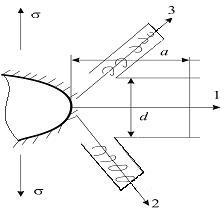
\includegraphics[width=0.4\textwidth]{assets/1319}
	\caption*{1-сурет - Жарықшықтың таралуының екі режимі: 1 -- иілгіш; 2, 3 -- нәзік тәрізді, a -- тереңдік және d -- жарықшақ мөлшері}
\end{figure}

\begin{figure}[H]
    \centering
    \begin{subfigure}[b]{0.22\textwidth}
        \centering
        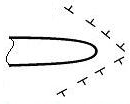
\includegraphics[width=\linewidth]{assets/1320}
		\caption*{а}
    \end{subfigure}
    \hfill
    \begin{subfigure}[b]{0.22\textwidth}
        \centering
        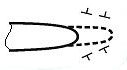
\includegraphics[width=\linewidth]{assets/1321}
		\caption*{б}
    \end{subfigure}
    \hfill
    \begin{subfigure}[b]{0.22\textwidth}
        \centering
        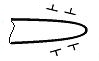
\includegraphics[width=\linewidth]{assets/1322}
		\caption*{в}
    \end{subfigure}
  \caption*{а - ақау ұшында дислокациялардың жиналуы; b -- критикалық дилатонның қалыптасуы; c- дилатон ыдырауынан кейінгі жарықшақтың ұзаруы}
  \caption*{2-сурет - Деструкцияның дайындық сатысындағы микрожарықшалардың өсу сұлбасы}
\end{figure}

\begin{multicols}{2}
Жалпы жағдайда сызаттардың үдемелі өсу сатысындағы бұзылу процесін
(деструкцияның дайындық кезеңі) келесідей көрсетуге болады 2-суретте
көрсетілген.

Бастапқы кезеңде дислокацияның бұзылуына және қозғалысына байланысты
материал құрылымының қайта құрылымдауы жүктемеге дейін ондағы ақаулардың
мезоскопиялық және құрылымдық деңгейлерінде орын алады. Дислокациялар
осы орталықтарға асығады 2а-суретте көрсетілген және олар кедергілерге
тап болған кезде бітеліп қалғанда, бұл аймақта серпімділік энергиясы
жиналады. Бұл денеде кездесетін ақаулардың жоғарғы жағында сыни
дилатондардың пайда болуына ықпал етеді 2б-суретте көрсетілген.

Осы уақыттағы микрожарықшалардың контуры материалдың зақымданбаған
бөлігінде критикалық дилатон түріндегі жалғасы бар құрылымдық ақаудың
контурымен анықталады.

Термиялық ауытқулардың әсерінен критикалық дилатондар жарылып ыдырайды,
эмбриональды жарықтар түзеді және бұрыннан бар ақаулармен біріктіріліп,
оларды ұзартады, 2в-суретінде көрсетілген. Жарылып, дилатон қоспалардан
дислокацияның босатылуын тудырады және стресс релаксациясы пайда болады.

Шекаралық массивтің таужыныстарының қатаюы (цементтеу, тау жыныстарының
химиялық қатаюы және т.б.) тау жыныстарының созылу беріктігінің
жоғарылауына және қазбалар маңындағы жарықшақ аймақтарының азаюына
немесе жойылуына әкеледі. Егер өңделген жыныс массасының беріктігі
шекаралық массаға әсер ететін кернеулерден үлкен болса, онда қирау
болмайды және кеңею жойылады.

Орын ауыстыруды есептеу бағдарламасы. Күтілетін жылжуларды болжауға
арналған жоғарыда сипатталған математикалық аппарат «КМС-Ш» (шахталар
үшін орын ауыстыруды модельдеу кешені). Бағдарлама есептеуде
қолданылатын коэффициенттер мен тұрақтылардың параметрлерін енгізуден
және программаның интерфейстік бөлігін инициализациялаудан басталады.

Келесі қадам қолайлы мәндер мен деректердің дұрыстығын бақылайтын
интерфейсті пайдаланып интерактивті деректерді енгізу болып табылады.

Бағдарламаға бастапқы деректер ретінде келесі көрсеткіштер енгізіледі:

\begin{itemize}
\item
  даму тереңдігі, м;
\item
  тау жыныстарының көлемдік салмағы, кН/м\textsuperscript{3};
\item
  қабаттардың қалыңдығын және сәйкес қабаттың физикалық-механикалық
  қасиеттерін (қысылу және созылу беріктігі, адгезия коэффициенті және
  т.б.) көрсететін жүргізіліп жатқан қазбаның геологиялық қимасы;
\item
  жыныс қабатының еңіс бұрышы, град;
\item
  қазбаның көлденең қимасының пішіні және оның геометриялық өлшемдері,
  м.
\end{itemize}

{\bfseries Нәтижелер мен талқылау.} Күтілетін жылжуларды сандық модельдеу
«АрселорМиттал Теміртау» АҚ КД Саранская кенішіндегі
50к\textsubscript{10}-1 шығыс желдеткіш еңісі мысалында қарастырылады.
Қазба 428-554 м тереңдікте, 100 бұрышта жүргізіледі. Қазбаның ұзындығы
630 м, орналасқан жеріндегі тігістің жалпы қалыңдығы 4,65 м.
К\textsubscript{10} тігістің құрылымы күрделі болып табылады. Қалыңдығы
0,05-1,17 м, көміртекті аргиллит пен қалыңдығы 0,01-0,04 м аргиллит
қабаттарымен бөлінген 9 көмір қаптамасының К\textsubscript{10} қабаты
көмір мен газдың кенеттен бөлінуінен қауіпті қабатқа жатады, тереңдігі
300 м. Қабат газ бен шаңның әсерінен қауіпті, өздігінен жануға бейім.

Қабаттың негізгі төбесінде құмтастар (m=23,7-29,56 м, f=60 МПа) бар.
Тікелей төбе қалыңдығы 1,24-2,09 м (f = 25 МПа) балшық тастармен
ұсынылған. Жалған төбесі көміртекті балшықтан, балшықтан тұрады,
қалыңдығы 0,45 м (f = 15 МПа).

Қабат топырағында қалыңдығы 5,25-6,35 м (f=20-25 МПа), тұрақсыз,
көтерілуге бейім аргиллиттер бар. Болжалды су ағыны 5
м\textsuperscript{3}/сағ дейін жетеді.

Қазбаны бекіту үшін 0,8 м қадаммен анкер тірегі қолданылады. Қазбаның 1
м жеріндегі анкерлер саны төбеде -- 12, бүйірлерде -- 6.

KMS-Ш бағдарламасын {[}5, 6{]} пайдалана отырып, контур массивінің
келесі күтілетін орын ауыстырулары алынды:

\begin{itemize}
\item
  қазбаның төбесінде -- 200 -- 300 мм;
\item
  қазбаның табанында -- 500 -- 650 мм;
\item
  қазбаның бүйірлерінде -- 150 -- 200 мм.
\end{itemize}

Модельдеу нәтижелерін және нақты орын ауыстыруларды салыстыру үшін ПК10,
18, 21, 32, 52, 59 пикеттерде бет ілгерілеуіне қарай бақылау станциялары
орнатылды.

Оң жақтан орын ауыстыруларды талдау 3а суретте көрсетілген деформацияның
интенсивті кезеңі бақылау эталондарын орнату сәтінен бастап бірінші айда
болатынын көрсетеді. Бірінші айда ығысу мөлшері 7 мм болды. Келесі
айларда ешқандай ауысым байқалмады.

Шахтаның оң жағында бірінші айда контурлық массивтің жыныстарының
қарқынды ығысулары байқалды. Максималды орын ауыстыру мәндері 3 мм
болды. Келесі айларда ауысым байқалмады.

3b-суретте желдеткіш еңістің төбесі жыныстарының жылжуының даму
динамикасы көрсетілген, одан барлық жылжулардың бірінші ай ішінде
болғанын көруге болады. Келесі айларда толық тоқтағанға дейін ығысу
қарқындылығының төмендеуі байқалады. Максималды орын ауыстыру мәндері 3
мм-ден аспады, бұл таңдалған тірек параметрлерінің тиімділігін
көрсетеді.
\end{multicols}

\begin{figure}[H]
    \centering
    \begin{subfigure}[b]{0.45\textwidth}
        \centering
        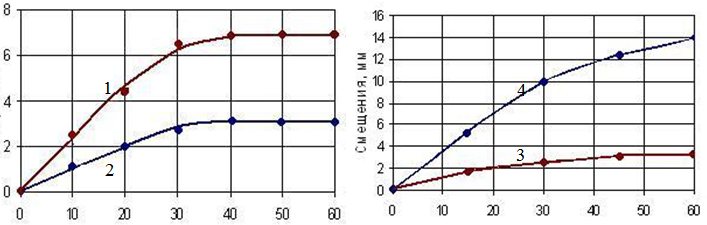
\includegraphics[width=\linewidth]{assets/1323}
		\caption*{тәулік, ұзақтығы}
		\caption*{a}
    \end{subfigure}
    \hfill
    \begin{subfigure}[b]{0.45\textwidth}
        \centering
        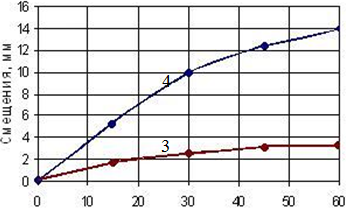
\includegraphics[width=\linewidth]{assets/1323.1}
		\caption*{тәулік, ұзақтығы}
		\caption*{b}
    \end{subfigure}
  \caption*{3-сурет - Тау жыныстарының оң (1) және сол (2) жағындағы жылжулары (а), төбе жыныстары (3) және табан (4) қазба (b)}
\end{figure}

\begin{multicols}{2}
Табандардың көтерілуін талдау бірінші айдағы ең жоғары ығысу мәндері 10
мм-ден аспайтынын көрсетті. Келесі айда қарқындылықтың төмендеуі
байқалды және максималды ығысулар 4 мм-ден аспады. Алынған ығысу
мәндерін тікелей табанда 5,25-6,35 м (f = 20-25 МПа) тұрақсыз,
көтерілуге бейім лай тастардың болуымен түсіндіруге болады. Тұтастай
алғанда, барлық пикеттер үшін орын ауыстыруларды талдау белгілі бір
дәрежеде жалпы сипатта және 4-суретте қарастырылған мысалға ұқсас.
\end{multicols}

\begin{figure}[H]
    \centering
    \begin{subfigure}[b]{0.45\textwidth}
        \centering
        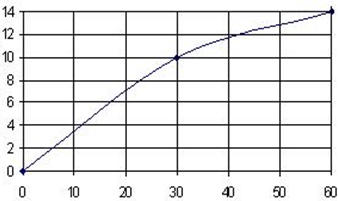
\includegraphics[width=\linewidth]{assets/1324}
		\caption*{тәулік, ұзақтығы}
		\caption*{a}
    \end{subfigure}
    \hfill
    \begin{subfigure}[b]{0.45\textwidth}
        \centering
        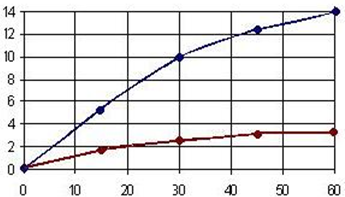
\includegraphics[width=\linewidth]{assets/1325}
		\caption*{тәулік, ұзақтығы}
		\caption*{b}
    \end{subfigure}
  \caption*{4-сурет - Қазбаның (а) және табандардың (b) жыныстарының жылжуының даму динамикасы}
\end{figure}

\begin{multicols}{2}
Анкерлік тірек пайдаланылмаған аймақ үшін контур массивінің жылжуын
есептеу алынған мәндер ± 7,2\% орташа квадраттық қателікпен байқалған
мәндермен сәйкес келетінін көрсетті.

Анкерлік тірек орнатылған аймақ үшін нақты нәтижелермен салыстырғанда
есептеу нәтижелерін ескере отырып, болжамды орын ауыстырулардың мәндері
нақтыдан үлкен мәндер реті екенін көрсетеді. Бұл жыныс болттарын
пайдалану күтілетін жылжуларды бірнеше есе азайтады дегенді білдіреді.

Анкерлік тірек болған кезде төбенің жылжуының қарқындылығы 8 мм, яғни.

\[b_{0} = \frac{8}{\ln(30 + 1)} = 2,33 \text{мм/ тәулік.}\]

Егер бірінші айдағы максималды күтілетін орын ауыстыруды 300 мм деп
алсақ, онда ығысу қарқындылығы мынаған тең болуы керек:

\[b_{0} = \frac{300}{\ln(30 + 1)} = 87,36 \text{мм/ тәулік.}\]

Көріп отырғаныңыздай, анкерлік болттардың жұмысының арқасында жылжу
қарқындылығы 40 есеге жуық азаяды.

Анкерлердің санын және олардың жүк көтергіштігін ескере отырып,
бекітілген және бекітілмеген жұмыстардың орын ауыстыру мәндері
арасындағы байланысты алуға болады (19):

\begin{equation}
U_{ф} = \Delta b_{0}U_{pc},
\end{equation}

мұнда \(\Delta b_{0} = \frac{b_{0}^{\text{Ф}}}{b_{0}^{\text{РАС}}}\) -- нақты орын
ауыстыру қарқындылығының есептелгенге қатынасы

немесе анкерді қолдану есебінен орын ауыстырулар

қарқындылығының төмендеуі қолдау көрсету.

Өз кезегінде, ығысу қарқындылығының төмендеуін критерий түрінде
көрсетуге болады:

\begin{equation}
\Delta b_{0} = f(P_{\text{анк}},N_{\text{анк}}),
\end{equation}

мұнда \(P_{\text{анк}}\) -- анкердің жүк көтергіштігі, т;

\(N_{\text{анк}}\) -- анкер саны, шт.

Ығысулардың қарқындылығы мен тіректің көтергіштігі арасындағы байланысты
анықтау үшін тіректің көтеру қабілетін өзгерту және әр жағдай бойынша
орын ауыстыруларды өлшеу арқылы әрі қарай зерттеулер жүргізу қажет.

Есептелген аналитикалық мәндерді сандық әдіспен алынған мәліметтермен
салыстыра отырып, олардың жинақтылығы туралы қорытынды жасауға болады:

\begin{itemize}
\item
  далалық өлшемдер мен аналитикалық әдіс арасындағы төбедеғі
  қозғалыстарды есептеу қателігі шамамен 2\% құрайды;
\item
  сандық және аналитикалық әдістерді қолдана отырып, эксперименттік
  мәліметтер арасындағы жақтардағы орын ауыстыруларды есептеу қателігі
  шамамен 6\% құрайды;
\item
  аналитикалық жолмен алынған табандағы қозғалыстар табиғи жағдайда
  алынған қозғалыстардан 2,8 есе көп.
\end{itemize}

Біртекті емес массивтегі тау жыныстарының деформацияланған күйін
реологиялық модель бойынша өңдеу, дайындық, капиталдық және т.б.,
кезінде тірек параметрлерін белгілей отырып модельдеу тек тау-кен
жұмыстарының әсерінен өндірісті жүргізу мен ұстаудың геомеханикалық
шарттарын ескере отырып мүмкін болады.

Геологиялық, тау-кен-техникалық және технологиялық пайдалану жағдайлары,
тау-кен жұмыстарын басқару схемалары:

\begin{itemize}
\item
  жұмыс тереңдігі, м; тік және көлденең жүктемелер,
  кН/м\textsuperscript{2}; Пуассон қатынасы {[}8,9{]}.
\end{itemize}

Массивтің тау-кен-геологиялық қасиеттеріне мыналар жатады:

\begin{itemize}
\item
  қабат сипаттамалары;
\item
  қабат төбесінің ординаты;
\item
  сәйкес жыныс қабатының адгезия коэффициенті;
\item
  ішкі үйкеліс бұрышы;
\item
  бір осьті қысу күші, МПа;
\item
  созылу беріктігі, МПа;
\item
  қабаттардың көкжиекке еңкею бұрышы.
\end{itemize}

Шахта контурларының ығысуы мен бұзылуының сандық нәтижелері 6-суретте
көрсетілген графикалық және мәтіндік формада берілген.

Бастапқы деректер: игеру тереңдігі -- 800 м; тік жүктеме -- 10
кН/м\textsuperscript{2}; көлденең жүктеме -- 10 кН/м\textsuperscript{2};
қазбаның көлденең қимасының пішіні тікбұрышты; жоғарғы жағындағы ені
(төменгі) -- 6,0 м; қазба биіктігі -- 4,0 м.

Нәтижесінде есептелген орын ауыстырулар: төбесі -- 0,272 м; табан --
0,276 м; жақтары -- 0,236 м.

Игеру қазбаларының айналасындағы шекаралық массивтегі тау жыныстарының
қабаттарының жылжу процесінің дамуына әртүрлі факторлардың әсерін
анықтау үшін орын ауыстыруларды модельдеуге арналған компьютерлік
бағдарламаны пайдаланып сандық тәжірибені қолдануға болады {[}10,11{]}.

Өндіріс орындарының жанындағы тау жыныстарының кернеулі-деформациялық
күйінің параметрлерін салыстырмалы бағалау үшін тау-кен геологиялық
жағдайларға байланысты шекаралық массивтің орын ауыстыруы.
\end{multicols}

\begin{figure}[H]
    \centering
    \begin{subfigure}[b]{0.45\textwidth}
        \centering
        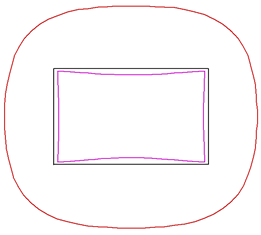
\includegraphics[width=0.8\linewidth]{assets/1333}
		\caption*{тәулік, ұзақтығы}
		\caption*{a}
    \end{subfigure}
    \hfill
    \begin{subfigure}[b]{0.45\textwidth}
        \centering
        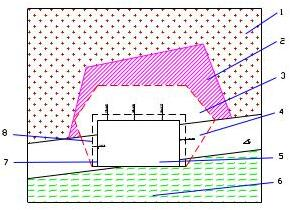
\includegraphics[width=\linewidth]{assets/1334}
		\caption*{тәулік, ұзақтығы}
		\caption*{b}
    \end{subfigure}
  \caption*{а -- қираулар мен ығысулар контурларының схемасы; b -- есеп
айырысуларға түсініктеме. 1 -- төбе жыныстары; 2 -- серпімді деформация аймағы; 3 және 4 --
қазбаның төбесі мен бүйіріндегі серпімсіз деформациялар аймақтары; 5 --
қазба қуысы; 6 -- табан жыныстары; 7 және 8 -- қазбаның пайдалану және
бастапқы контуры.}
  \caption*{5-сурет - Есептеу нәтижелері туралы есептің мысалы}
\end{figure}

\begin{multicols}{2}
Дамуын зерттеудің аналитикалық және тәжірибелік әдістері қолданылды.
Жылжулардың дамуына әсер ететін негізгі фактор жұмыстың тереңдігіне
байланысты тау жыныстарының қысымы болып табылады.

Орташа біртекті массивте бір жұмыс үшін есептеулер жүргізілді, Қарағанды
көмір бассейні үшін тау жыныстарының бір осьтік сығу беріктігі 24 МПа.

Өңдеудің көлденең қимасының пішіні доға тәріздес, ені -- 5,57 және
биіктігі -- 3,55 м, қазбалардың батыру тереңдігі 400 м-ден 800 м-ге
дейін өзгерді (Қарағанды көмір бассейнінің шахталары үшін тереңдік
интервалы).

Контур массивінің жылжуларының жұмыс тереңдігіне аналитикалық
тәуелділігі 6а-суретте көрсетілген. Бүйірлік итеру коэффициентінің мәні
1,0 деп қабылданады.

Қарастырылған тереңдік интервалы үшін контурлық массивтің тіреусіз
жұмыстың төбе жағынан күтілетін жылжулары мен 6а-суретте көрсетілген
жұмыс тереңдігі арасындағы сызықтық байланыс орнатылды, формуламен
өрнектеледі (21):

\begin{equation}
U_{\text{ожид}} = 0,3093Н - 21,322,\ \text{при \emph{r} = 0,97.}
\end{equation}

Кен қазбаларының шекаралық массасының ығысуына әсер ететін маңызды
фактор тәжірибеде Қарағанды көмір бассейніне тән шектерде (10-40 МПа)
өзгерген тау жыныстарының беріктігі болып табылады.

Контурлық жыныс массасының жылжуларының беріктікке экспоненциалды
тәуелділігі анықталды, формуламен өрнектеледі (22):

\begin{equation}
U_{\text{ожид}} = 1294,4е^{- 0,1003\sigma_{\text{сж}}},\ \text{кезінде \emph{r} = 0,96.}
\end{equation}

Контурлық массив таужыныстарының төбе жағынан ығысуларының олардың бір
осьтік сығымдалу беріктігіне тәуелділігі 6\emph{b}-суретте көрсетілген.

6\emph{b}-суреттен максималды ығысулар тау жыныстарының минималды
беріктігіне сәйкес келетіні, сәйкесінше ең жоғары тау жыныстарының
беріктігі ең аз ығысуларға сәйкес келетіні шығады.
\end{multicols}

\begin{figure}[H]
    \centering
    \begin{subfigure}[b]{0.45\textwidth}
        \centering
        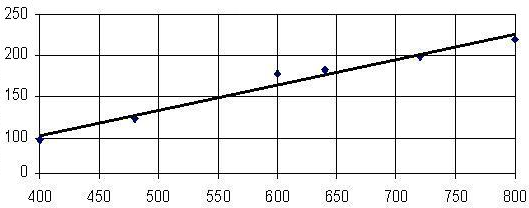
\includegraphics[width=\linewidth]{assets/1337}
		\caption*{тәулік, ұзақтығы}
		\caption*{a}
    \end{subfigure}
    \hfill
    \begin{subfigure}[b]{0.45\textwidth}
        \centering
        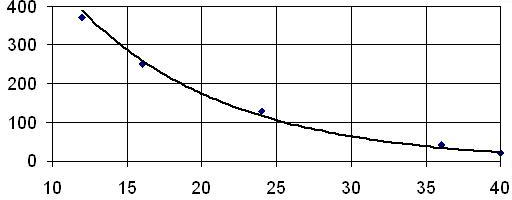
\includegraphics[width=\linewidth]{assets/1338}
		\caption*{тәулік, ұзақтығы}
		\caption*{b}
    \end{subfigure}
  \caption*{6-сурет - Контурлық массив таужыныстарының жылжуларының жұмыс тереңдігіне тәуелділігі (а) және олардың төбе жағынан бір осьті сығуға беріктігі (b)}
\end{figure}

\begin{multicols}{2}
{\bfseries Қорытынды.} Тау жыныстарының қопсыту коэффициентін азайту
жөніндегі ұсынымдар (дилатансия) мынадай параметрлерге әсер етумен
алынуы мүмкін. Деформациялау жылдамдығының артуы жыныс беріктігі шегінің
және серпінді энергияның өсуіне әкеледі, бұл қазбаға жақын қирау
аймағының пайда болу ықтималдығын төмендету тұрғысынан қолайлы және егер
есептік кернеулер жыныс беріктігінің шегінен артық болса, жыныстардың
қопсытылуының ұлғаюына әкеледі. Егер қирау аймақтары қалыптасатын болса,
ал бұл қазба жүргізілген жыныстардың қасиеттеріне байланысты болса,
жарықтар қабырғаларының жылжуы есебінен дилатанцияны төмендету үшін
жыныстардың деформация жылдамдығын төмендету қажет, бұл жыныстарды
жалаңаштағаннан кейін бірден тау-кен бекітпесін орнатумен қол жеткізілуі
мүмкін.

Кернеудің өсуі қазбаның жату тереңдігімен анықталады. Қазба контурынан
массивтің тереңдігіне алшақтау арқылы жарықтардың аралас беттерінің орын
ауыстыруынан дилатация ықтималдығы төмендейді.

Жыныстарды қопсыту кернеу шоғырлануын және кернеудің төмен мәнін
болдырмайтын қазбалардың көлденең қимасының нысанын қолдану есебінен
азайтылуы мүмкін.

Жыныстар құрылымының сипаттамасы жыныстардың бұзылуы кезінде үлкен жаққа
және нығаюы кезінде аз жаққа өзгереді. Екі жағдайда да жыныс
беріктігінің шегіне әсер етеді. Беріктік шегінің төмендеуі қирау
аймағының ұлғаюына әкеледі, ал пластикалық қасиеттердің ұлғаюы
жинақталған серпінді энергияның төмендеуіне және жарықтың қарама-қарсы
беттерінің орын ауыстыруынан дилатансия ықтималдығына әкеледі.

Контур жанындағы массив жыныстарының нығаюы (цементтеу, жыныстардың
химиялық нығаюы және т.б.) жыныстардың беріктігі шегінің ұлғаюына және
қазбаға жақын қирау аймағының азаюына немесе жойылуына әкеледі. Егер
жыныстардың өңделген массивінің беріктігі контур жанындағы массивте
әрекет ететін кернеулерден артық болған жағдайда, қираулар болмайды және
дилатансия болмайды.
\end{multicols}

\begin{center}
{\bfseries Әдебиеттер}
\end{center}

\begin{noparindent}
1.Demin W., Demina, Т. Deminа, Steflyuk Y. Enhancement of coal seams and
mined-out areas degassing

productivity (статья). Progressive
  Technologies of Coal, Coalbed Methane, and Ores Mining--Bondarenko,
  
  Kovalevs'ka \& Ganushevych (eds), Taylor \& Francis Group, London,
  2014. - С. 209-215.

2.Демин В.Ф., Демина Т.В., Кайназаров А.С., Кайназарова А.С. Оценка
  эффективности применения технологических схем проведения горных
  выработок для повышения устойчивости их контуров// Устойчивое развитие
  горных территорий. -- 2018. - Т.10. - № 4 (38). - C. 606 - 617. DOI
  10.21177/1998-4502-2018-10-4-606-616

3.Цай Б.Н., Бондаренко Т.Т., Бахтыбаев Н.Б. Одилатансии горных пород //
  Вестник КазНТУ. -2008. - № 5. -С. 45 -- 50.

4.Ставрогин А.Н., Протосеня А.Г. Механика деформирования и разрушения
  горных пород. -- М.: Недра, 1992. -- 224 с.

5.Демин, В.Ф. Технология крепления выработок на основе оценки
  напряженно-деформированного состояния породно-анкерной конструкции :
  монография / В. Ф. Демин, Т. В. Демина, А. Д. Каратаев. - Караганда :
  ТОО "Арко", 2015. - 200 с. - (Рейтинг). - ISBN 978-601-204-240-5

6.Демин В.Ф., Демина Т.В. Технология повышения устойчивости
  геомеханической системы «анкерная крепь-слоистый массив
  пород»:монография. -Караганда, изд-во «Арко». 2015. -204 с.

7.Зейнуллин А.А., Кайназарова А.С., Кайназаров А.С. и др. Оценка
  способов поддержания горных выработок на основе применения анкерной
  крепи на шахтах Карагандинского угольного бассейна//Уголь. -- 2021. --
  №2. -- С. 4-9. DOI 10.18796/0041-5790-2021-2-4-9

8.Алиев С.Б., Демин В.Ф., Кайназаров А.С., Милитенко Н.А. Оценка
  состояния приконтурного горного массива на сопряжении лавы с
  примыкающей выемочной выработкой //Уголь. -- 2023. -- №1. -- С. 35-39.
  DOI 10.18796/0041-5790-2023-1-35-39

9.Абеуов. Е.А, Демин В.Ф., Кайназаров А.С. Развитие деформаций в почве
  при установке припочвенной анкерной крепи// Промышленность Казахстана,
  Алматы, 2019, №2(106), С. 74 -77.

10.Голик В.И. Оптимизация технологии разработки маломощных пологих рудных
  тел на геомеханической основе// Известия Тульского государственного
  университета. Науки о Земле. 2016. № 4. С. 139-152.

11.Matayev A.K., Kainazarova A.S. et al. Research into rock mass
  gejvtchanical sition in the zone of stope operations influence at the
  10th Anniversary of Kazakhstan's Independence mine // Mining of
  Mineral Deposits. -- 2021. -- Vol.~15, Iss. 1. -- P. 103-111. DOI
  10.33271/mining15.01.103
\end{noparindent}

\begin{center}
{\bfseries References}
\end{center}

\begin{noparindent}
1. Demin W., Demina, T. Demina, Steflyuk Y. Enhancement of coal seams
and mined-out areas degassing productivity (stat\textquotesingle ya).
Progressive Technologies of Coal, Coalbed Methane, and Ores
Mining--Bondarenko,

Kovalevs'ka \& Ganushevych (eds), Taylor \& Francis
Group, London, 2014. - S. 209-215.

2. Demin V.F., Demina T.V., Kainazarov A.S., Kainazarova A.S. Otsenka
effektivnosti primeneniya

tekhnologicheskikh skhem provedeniya gornykh
vyrabotok dlya povysheniya ustoichivosti ikh konturov// Ustoichivoe
razvitie gornykh territorii. -- 2018. - T.10. - № 4 (38). - C. 606 -
617. DOI 10.21177/1998-4502-2018-10-4-606-616 {[}in Russian{]}

3. Tsai B.N., Bondarenko T.T., Bakhtybaev N.B. Odilatansii gornykh porod
// Vestnik KazNTU. -2008. - № 5. -S. 45 -- 50. {[}in Russian{]}

4. Stavrogin A.N., Protosenya A.G. Mekhanika deformirovaniya i
razrusheniya gornykh porod. -- M.: Nedra, 1992. -- 224 s. {[}in
Russian{]}

5. Demin, V.F. Tekhnologiya krepleniya vyrabotok na osnove otsenki
napryazhenno-deformirovannogo sostoyaniya porodno-ankernoi konstruktsii
: monografiya / V. F. Demin, T. V. Demina, A. D. Karataev. - Karaganda :
TOO "Arko", 2015. - 200 s. - (Reiting). - ISBN 978-601-204-240-5 {[}in
Russian{]}

6. Demin V.F., Demina T.V. Tekhnologiya povysheniya ustoichivosti
geomekhanicheskoi sistemy «ankernaya krep\textquotesingle-sloistyi
massiv porod»:monografiya. -Karaganda, izd-vo «Arko». 2015. -204 s.
{[}in Russian{]}

7. Zeinullin A.A., Kainazarova A.S., Kainazarov A.S. i dr. Otsenka
sposobov podderzhaniya gornykh vyrabotok na osnove primeneniya ankernoi
krepi na shakhtakh Karagandinskogo ugol\textquotesingle nogo
basseina//Ugol\textquotesingle. -- 2021. -- №2. -- S. 4-9. DOI
10.18796/0041-5790-2021-2-4-9 {[}in Russian{]}

8. Aliev S.B., Demin V.F., Kainazarov A.S., Militenko N.A. Otsenka
sostoyaniya prikonturnogo gornogo massiva na sopryazhenii lavy s
primykayushchei vyemochnoi vyrabotkoi //Ugol\textquotesingle. -- 2023.
-- №1. -- S. 35-39.

DOI 10.18796/0041-5790-2023-1-35-39 {[}in Russian{]}

9. Abeuov. E.A, Demin V.F., Kainazarov A.S. Razvitie deformatsii v
pochve pri ustanovke pripochvennoi ankernoi krepi//
Promyshlennost\textquotesingle{} Kazakhstana, Almaty, 2019, №2(106), S.
74 -77. {[}in Russian{]}

10. Golik V.I. Optimizatsiya tekhnologii razrabotki malomoshchnykh
pologikh rudnykh tel na geomekhanicheskoi osnove// Izvestiya
Tul\textquotesingle skogo gosudarstvennogo universiteta. Nauki o Zemle.
2016. № 4. S. 139-152. {[}in Russian{]}

11. Matayev A.K., Kainazarova A.S. et al. Research into rock mass
gejvtchanical sition in the zone of stope operations influence at the
10th Anniversary of Kazakhstan's Independence mine // Mining of Mineral
Deposits. -- 2021. -- Vol. 15, Iss. 1. -- P. 103-111. DOI
10.33271/mining15.01.103
\end{noparindent}

\emph{{\bfseries Авторлар туралы мәліметтер}}

\begin{noparindent}
Қайназаров А.С. - техника ғылымдарының кандидаты, академик Қ. Сәтбаев
атындағы Екібастұз инженерлік-техникалық институты, Екібастұз,
Қазақстан, e-mail: armanayn@mail.ru;

Демин В.Ф. - техника ғылымдарының докторы, профессор, «Әбілқас Сағынов
атындағы Қарағанды техникалық университеті» КЕАҚ, Қарағанды, Қазақстан,
e-mail: vladfdemin@mail.ru;

Қайназарова А.С. - PhD докторы, академик Қ. Сәтбаев атындағы Екібастұз
инженерлік-техникалық институты, Екібастұз, Қазақстан, e-mail:
k.ainash.c@mail.ru;

Абрахман Е. А. -- докторант, НАО «Карагандинский технический университет
имени Абылкаса Сагинова», Казахстан, Караганда, e-mail:
yelnur.abdrakhman@mail.ru.
\end{noparindent}

\emph{{\bfseries Information about the authors}}

\begin{noparindent}
Kainazarov A.S. - Candidate of Technical Sciences, Ekibastuz Engineering
and Technical Institute named after

Academician K. Satpayeva, Kazakhstan, e-mail: armanayn@mail.ru;

Demin V.F. - Doctor of Technical Sciences, Professor, Abylkas Saginov
Karaganda Technical University NPJSC, Kazakhstan, e-mail:
vladfdemin@mail.ru;

Kainazarova A.S. -- Doctor PhD, Ekibastuz Engineering and technical
Institute named after academician K. Satpayev, Ekibastuz, Kazakhstan,
e-mail: k.ainash.c@mail.ru.

Abrahman E. A. - is a doctoral student, "Abilkas Saginov Karaganda
Technical University" NPJSC, Karaganda, Kazakhstan, e-mail:
yelnur.abdrakhman@mail.ru.
\end{noparindent}
